\chapter{Experiment Results}

This chapter presents the experimental results of the proposed OptiX-based SDF computation pipeline. We describe the testing methodology, analyze the time complexity and real-time performance compared to the PyMeshLab GPU implementation, and evaluate the visual quality of the computed SDF values.

\section{Testing Method}

The experiments were conducted on a system equipped with an NVIDIA RTX GPU using CUDA and OptiX RT Cores. Two implementations were benchmarked: the proposed OptiX-based pipeline and the PyMeshLab GPU implementation (VCGlib/OpenGL). Both implementations used identical SDF parameters: 64 rays per vertex, a cone angle of 150 degrees, depth peeling iterations = 10 (higher values are needed for bigger models, but we fixed it for the sake of testing the framework easier), and no outlier removal. The OptiX pipeline included full post-processing (log normalization and 3 iterations of anisotropic bilateral smoothing), while PyMeshLab produced raw SDF values without post-processing. Timing was measured using \texttt{std::chrono::high\_resolution\_clock} for OptiX and \texttt{time.perf\_counter()} for PyMeshLab, with visualization disabled in both cases.

After the smoothed SDF values are computed, the results are visualized and compared against the reference implementation. The final SDF values are visualized as vertex-colored heat maps using Polyscope, a 3D geometry processing viewer. The \texttt{turbo} colormap maps normalized SDF values from blue (thin) to red (thick). Three models are displayed simultaneously for comparison. The OptiX SDF represents the smoothed result from the proposed pipeline. The PyMeshLab SDF is the reference result computed using VCGlib's OpenGL rasterization with identical parameters ($R = 64$, $\theta_{\mathrm{cone}} = 150^\circ$). The Difference model shows the absolute per-vertex difference $|v_{\mathrm{optix}} - v_{\mathrm{pymeshlab}}|$ for accuracy assessment.

\section{Time Complexity and Real-Time Speed Comparison}

The time complexity analysis reveals fundamental differences between the two approaches. Let $V$ = number of vertices, $F$ = number of faces, $R$ = rays per vertex, $N$ = number of camera directions, $P$ = depth peeling iterations (the bigger the model, the more peeling iterations it needs), $I$ = smoothing iterations, and $k$ = average neighbors per vertex.

The OptiX pipeline has total complexity $O(V \times R \times \log F + F \log F)$, dominated by BVH construction and ray tracing. Each vertex independently shoots $R$ rays through the hardware BVH, with each ray traversing the BVH in $O(\log F)$. The VCGlib/MeshLab GPU approach has total complexity $O(N \times (F \times P + V))$, dominated by depth peeling across all camera directions. Each of the $N$ directions requires a full mesh render pass with $P$ depth peeling layers.

Despite the $\log F$ factor in OptiX, it outperforms VCGlib because: (1) OptiX launches $V$ threads in parallel with RT Cores handling ray-BVH traversal in hardware, while VCGlib requires $N$ draw calls with fixed overhead; (2) OptiX uses zero-copy CUDA device pointers with no host-device transfer, while VCGlib requires \texttt{glReadPixels} readback; (3) OptiX's post-processing adds negligible cost compared to ray tracing, while VCGlib has no post-processing at all.

Table~\ref{tab:benchmark} shows the benchmark results across 12 models, comparing the execution time of the PyMeshLab GPU implementation against the proposed OptiX pipeline. OptiX is faster across all models, with speedups ranging from 3.1x to 171x. The table lists each model name, its vertex count, the execution time for both implementations in seconds, and the resulting speedup factor.

\begin{table}[ht]
\centering
\begin{tabular}{@{}lrrrr@{}}
\toprule
\textbf{Model} & \textbf{Vertices} & \textbf{PyMeshLab (s)} & \textbf{OptiX (s)} & \textbf{Speedup} \\
\midrule
360.obj & 2,200 & 0.3228 & 0.0019 & 171.0x \\
9.obj & 2,639 & 0.4359 & 0.0084 & 51.6x \\
400.obj & 3,703 & 0.4004 & 0.0121 & 33.2x \\
76.obj & 5,923 & 0.5027 & 0.0106 & 47.6x \\
181.obj & 7,242 & 0.3128 & 0.0039 & 80.6x \\
118.obj & 9,153 & 0.3141 & 0.0047 & 66.3x \\
368.obj & 11,202 & 0.3217 & 0.0163 & 19.7x \\
112.obj & 13,628 & 0.8288 & 0.0229 & 36.1x \\
369.obj & 13,606 & 0.3772 & 0.0517 & 7.3x \\
158.obj & 14,587 & 0.3450 & 0.0069 & 50.0x \\
371.obj & 14,599 & 0.3097 & 0.0583 & 5.3x \\
Leaf.obj & 24,866 & 0.3827 & 0.1219 & 3.1x \\
\bottomrule
\end{tabular}
\caption{Performance benchmark: PyMeshLab GPU vs.\ OptiX}
\label{tab:benchmark}
\end{table}

PyMeshLab GPU has a approximately 0.3s base overhead regardless of model size, due to OpenGL context initialization, texture upload, and iterating over 128 camera directions. OptiX scales better as its ray tracing time grows proportionally with vertex count, while PyMeshLab's overhead is dominated by fixed-cost OpenGL operations.

\section{Quality Comparison}

The visual quality of the computed SDF values was evaluated by comparing the OptiX results against the PyMeshLab GPU reference. Each comparison shows the SDF heat map from both implementations and their absolute difference per vertex. Hot colors (red/yellow) indicate larger SDF values (thicker regions), while cool colors (blue) indicate thinner regions.

Figure~\ref{fig:quality_112} through Figure~\ref{fig:quality_368} show the comparison results for representative models. The OptiX pipeline produces SDF values that closely match the PyMeshLab reference, with the difference maps showing minimal variation. The OptiX SDF is much smoother than the PyMeshLab result due to the anisotropic bilateral smoothing applied in the post-processing stage, which reduces noise while preserving features.

\begin{figure}[ht]
\centering
\begin{tabular}{@{}c@{}}
\cellcolor{red!15}\textbf{OptiX} \\
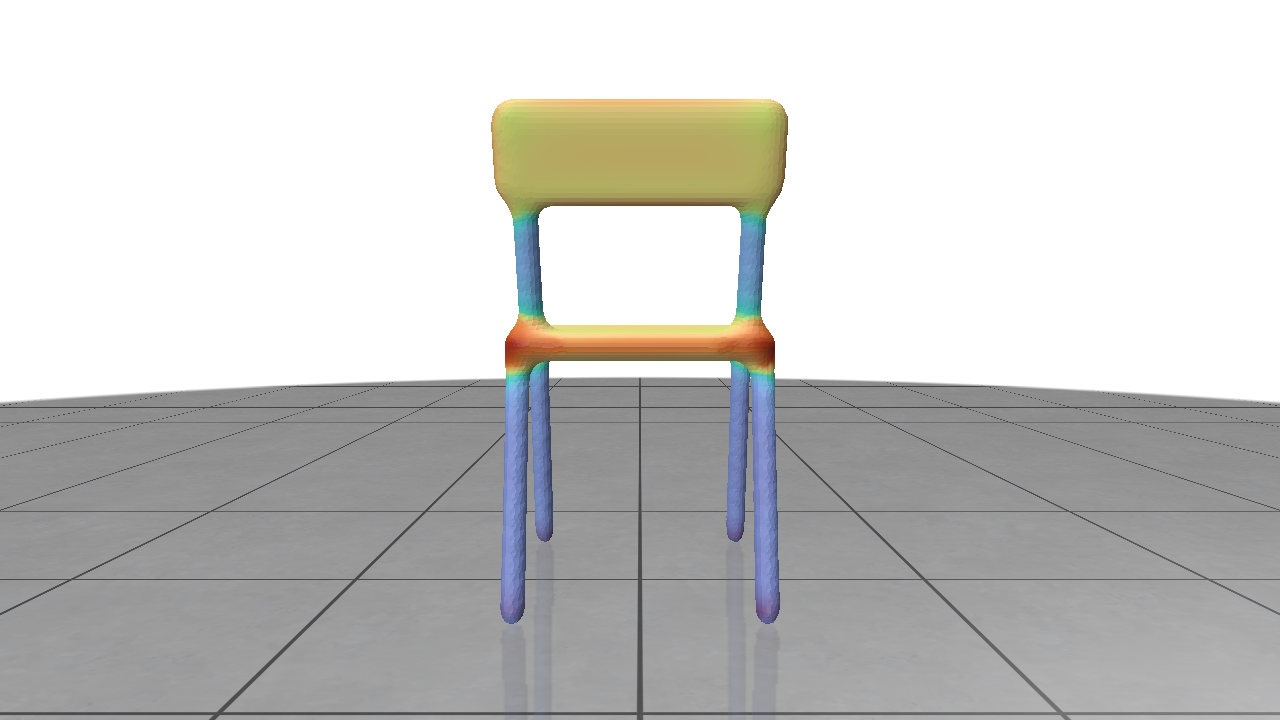
\includegraphics[width=0.65\textwidth]{../image/112_optix.png} \\
\cellcolor{green!15}\textbf{PyMeshLab} \\
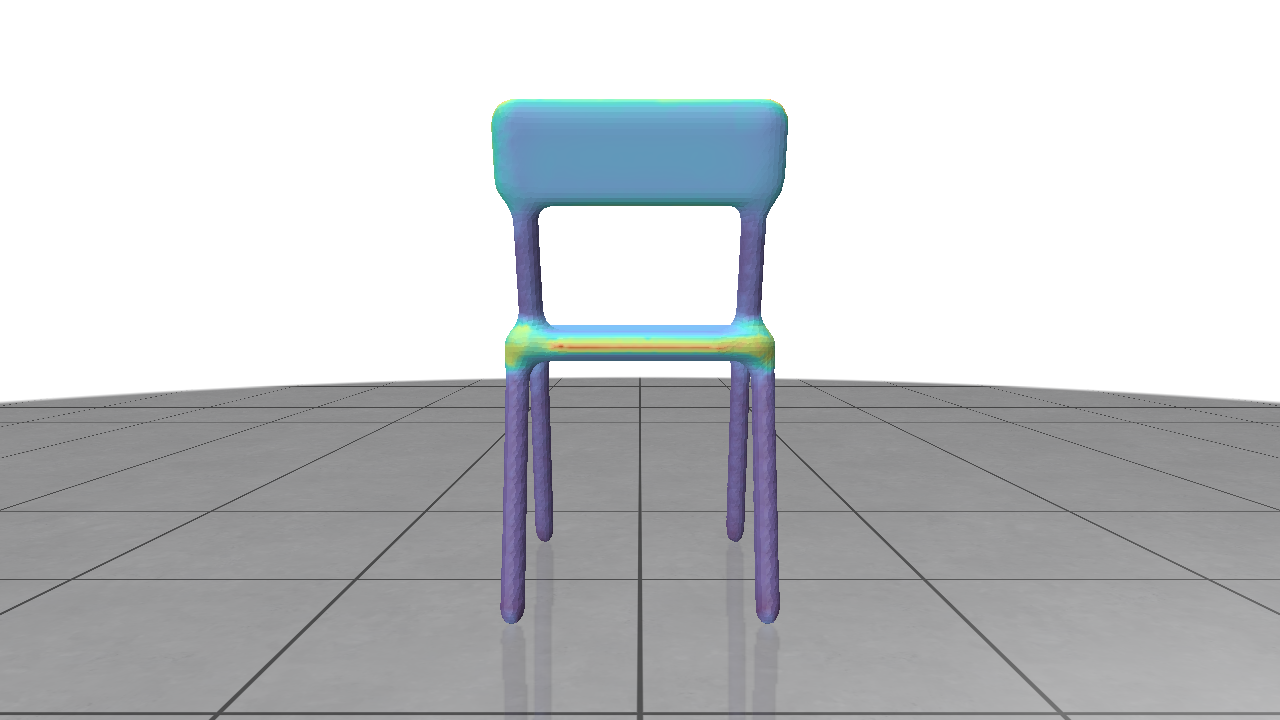
\includegraphics[width=0.65\textwidth]{../image/112_pymeshlab.png} \\
\cellcolor{blue!15}\textbf{Difference} \\
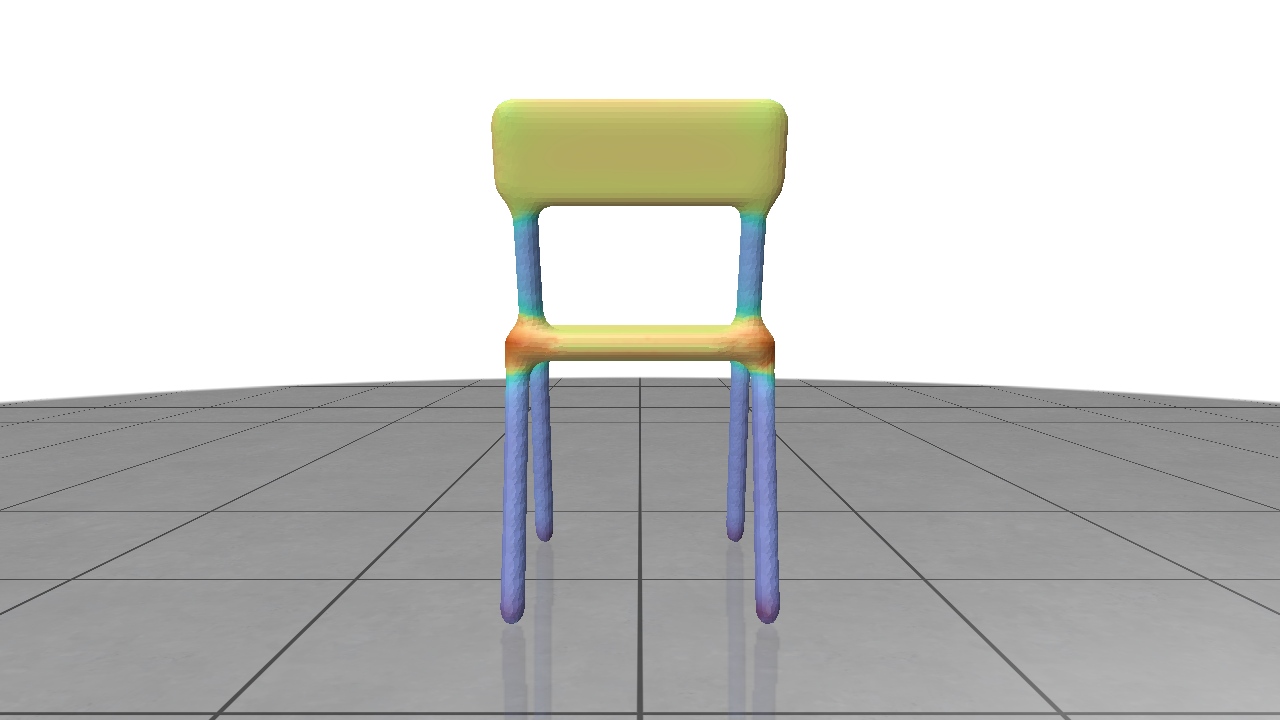
\includegraphics[width=0.65\textwidth]{../image/112_diff.png} \\
\end{tabular}
\caption{SDF quality comparison for model 112.obj (13,628 vertices)}
\label{fig:quality_112}
\end{figure}

Model 112 is one of the larger models in the dataset. The OptiX result shows a smooth, coherent heat map with well-defined thickness gradients across the surface. The PyMeshLab result exhibits slight noise in the thickness transitions. The difference map confirms that the discrepancy is minimal, with the largest deviations occurring at thin structural features where the bilateral smoothing in OptiX preserves edges more effectively.

\begin{figure}[ht]
\centering
\begin{tabular}{@{}c@{}}
\cellcolor{red!15}\textbf{OptiX} \\
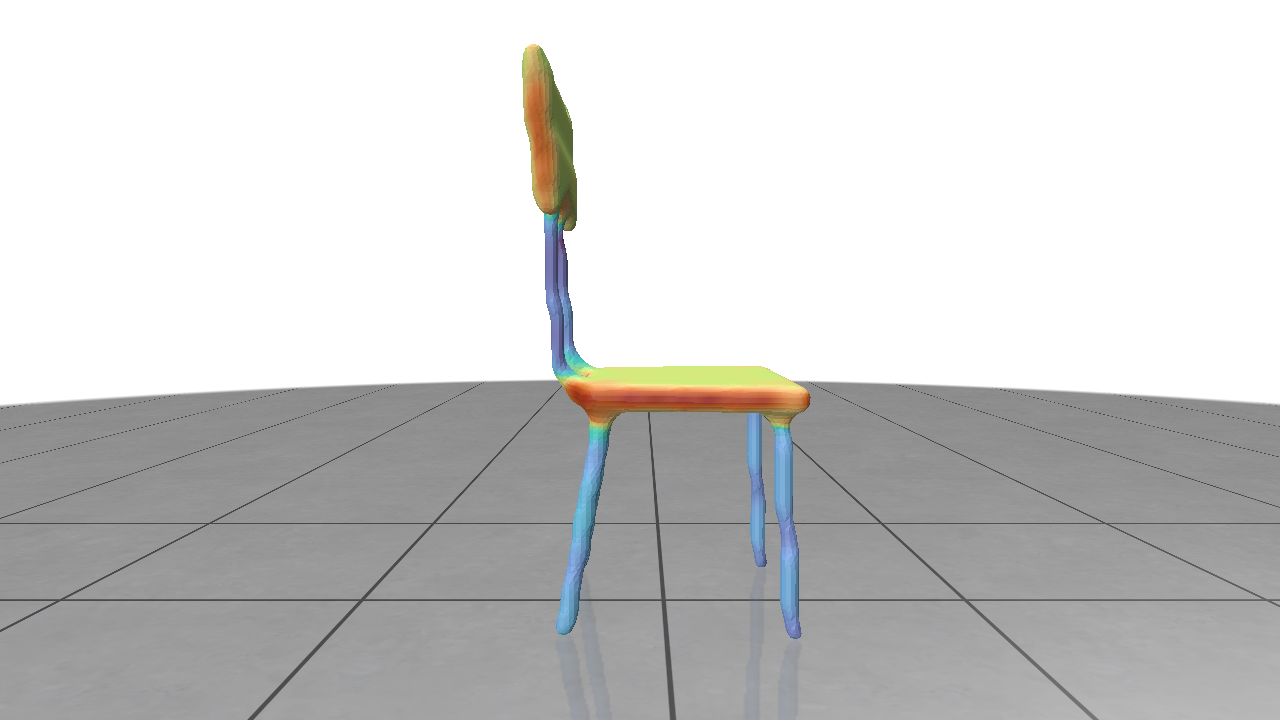
\includegraphics[width=0.65\textwidth]{../image/118_optix.png} \\
\cellcolor{green!15}\textbf{PyMeshLab} \\
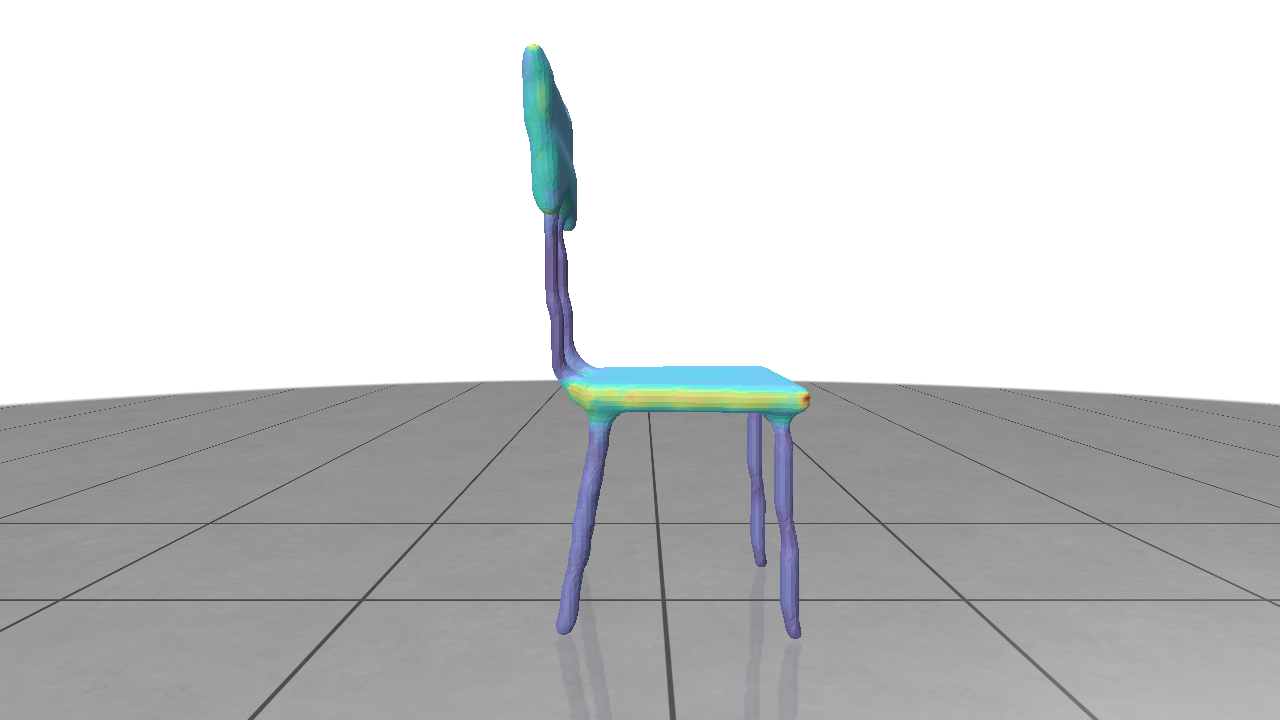
\includegraphics[width=0.65\textwidth]{../image/118_pymeshlab.png} \\
\cellcolor{blue!15}\textbf{Difference} \\
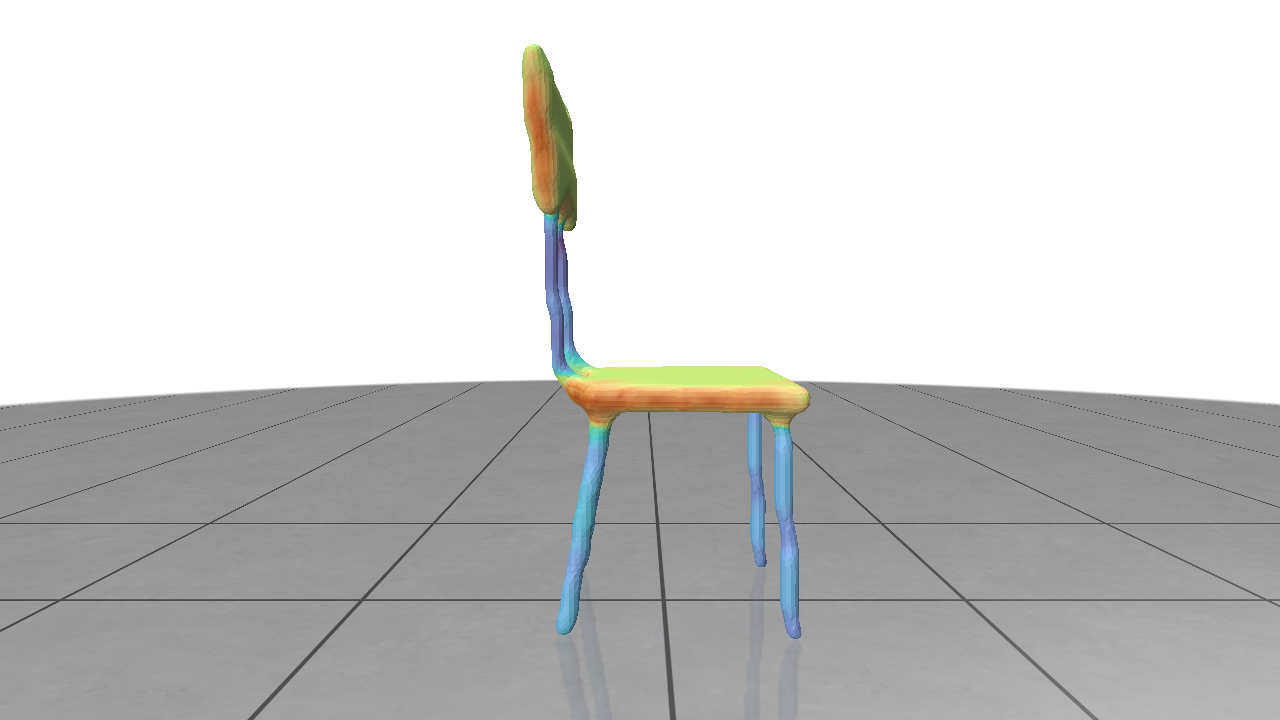
\includegraphics[width=0.65\textwidth]{../image/118_diff.png} \\
\end{tabular}
\caption{SDF quality comparison for model 118.obj (9,153 vertices)}
\label{fig:quality_118}
\end{figure}

Model 118 has a moderate vertex count and exhibits complex surface curvature. The OptiX heat map shows smooth thickness variation across curved regions, while the PyMeshLab result displays minor artifacts in areas of high curvature. The difference map indicates that both implementations agree on the overall thickness distribution, with discrepancies confined to local surface features.

\begin{figure}[ht]
\centering
\begin{tabular}{@{}c@{}}
\cellcolor{red!15}\textbf{OptiX} \\
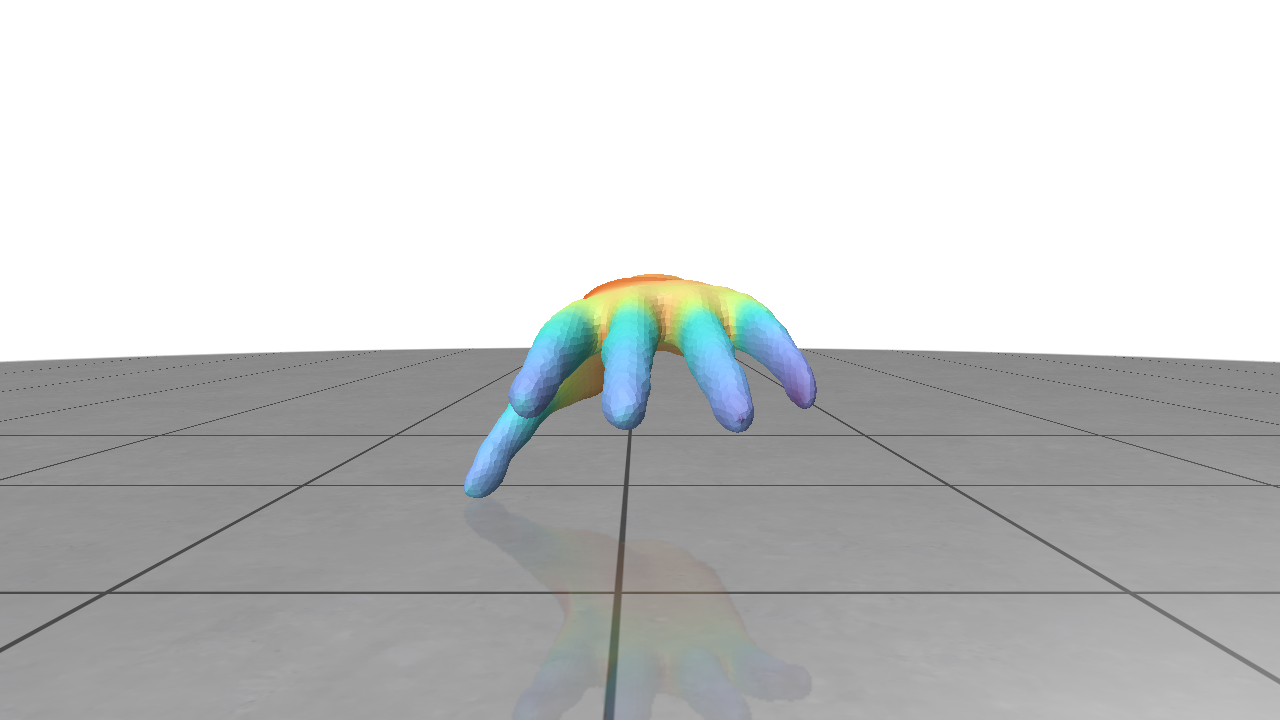
\includegraphics[width=0.65\textwidth]{../image/181_optix.png} \\
\cellcolor{green!15}\textbf{PyMeshLab} \\
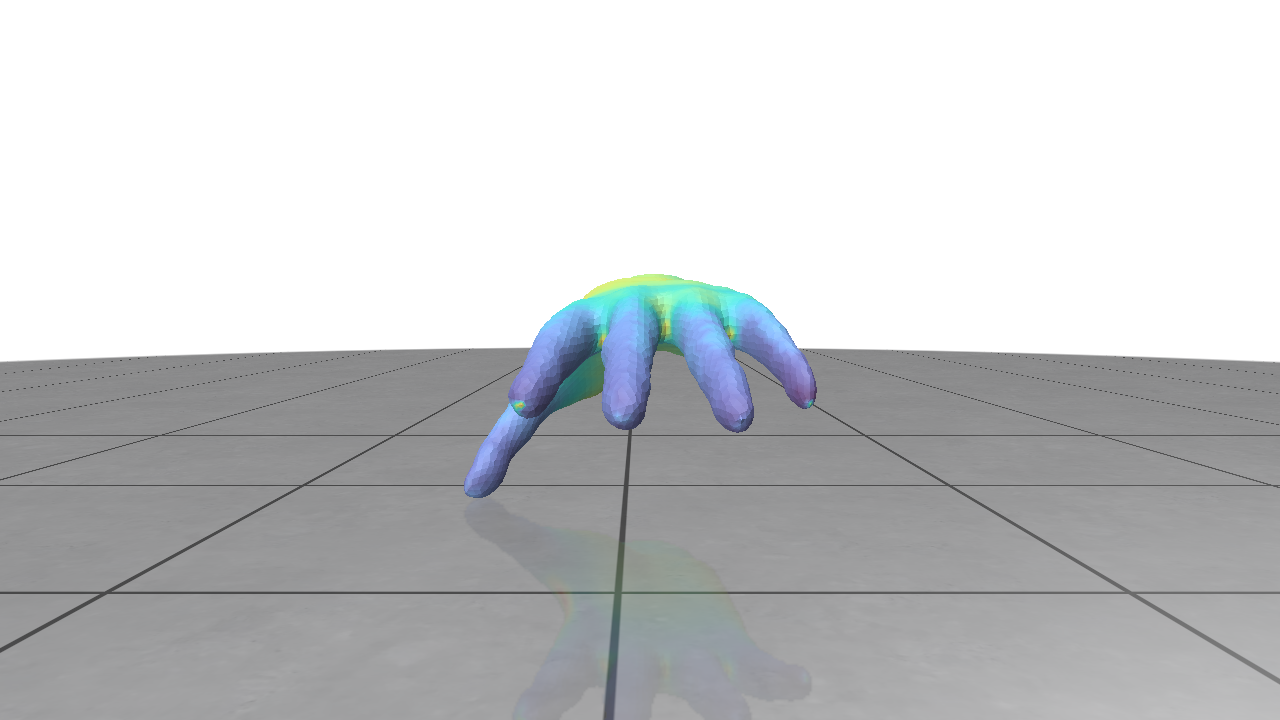
\includegraphics[width=0.65\textwidth]{../image/181_pymeshlab.png} \\
\cellcolor{blue!15}\textbf{Difference} \\
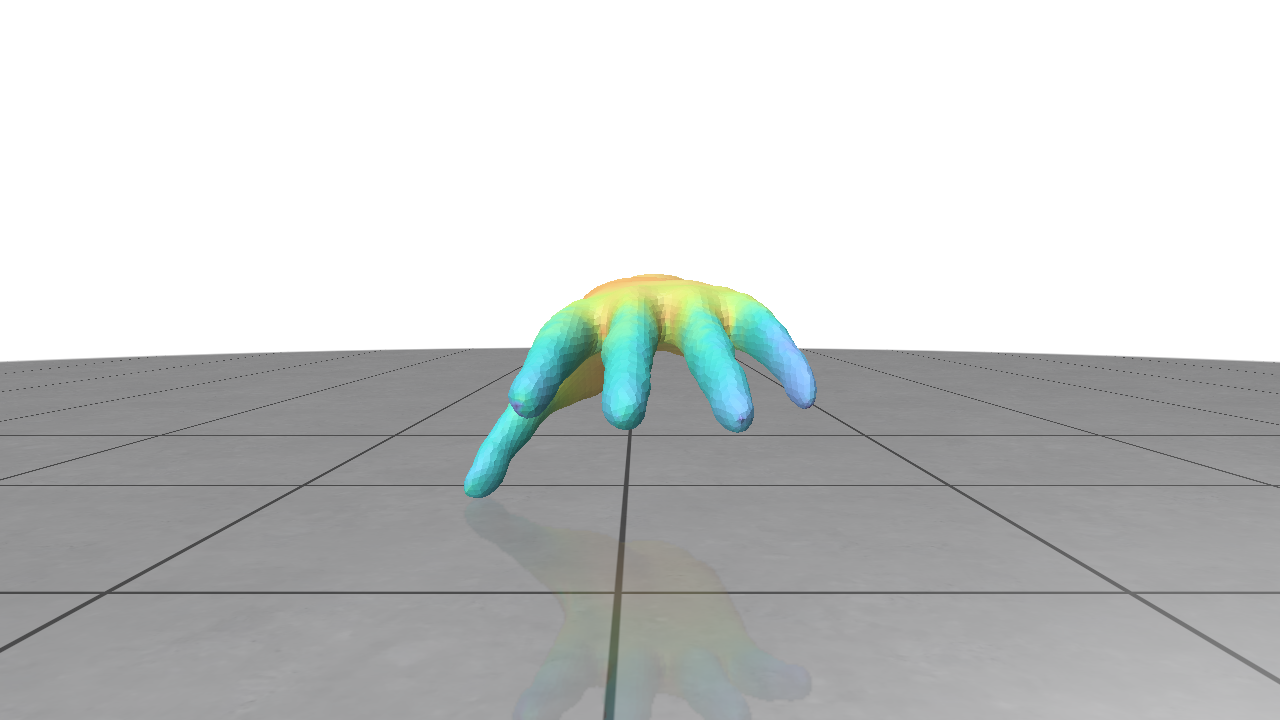
\includegraphics[width=0.65\textwidth]{../image/181_diff.png} \\
\end{tabular}
\caption{SDF quality comparison for model 181.obj (7,242 vertices)}
\label{fig:quality_181}
\end{figure}

Model 181 has 7,242 vertices and features a mix of smooth and sharp surface regions. The OptiX heat map captures smooth thickness gradients while preserving sharp transitions at feature edges. The PyMeshLab result shows comparable overall accuracy but with slightly more noise in flat regions. The difference map confirms that both implementations produce consistent SDF values, with the bilateral smoothing in OptiX contributing to a cleaner result.

\begin{figure}[ht]
\centering
\begin{tabular}{@{}c@{}}
\cellcolor{red!15}\textbf{OptiX} \\
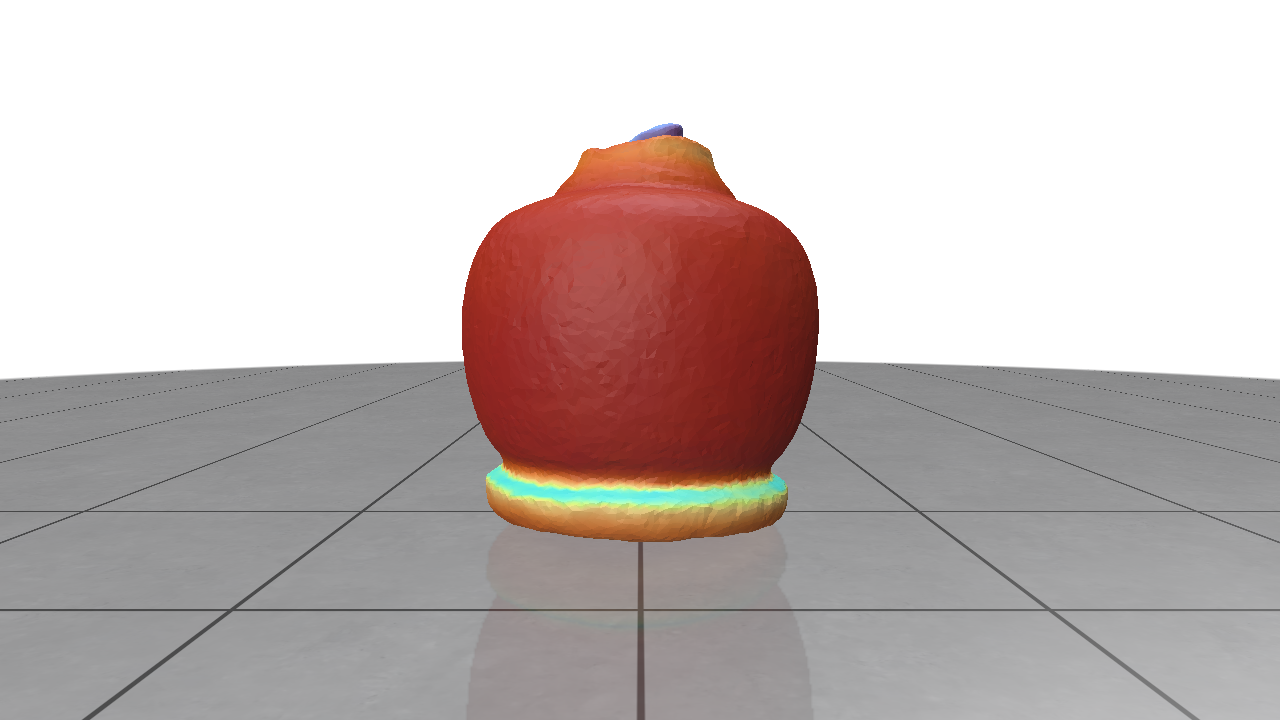
\includegraphics[width=0.65\textwidth]{../image/368_optix.png} \\
\cellcolor{green!15}\textbf{PyMeshLab} \\
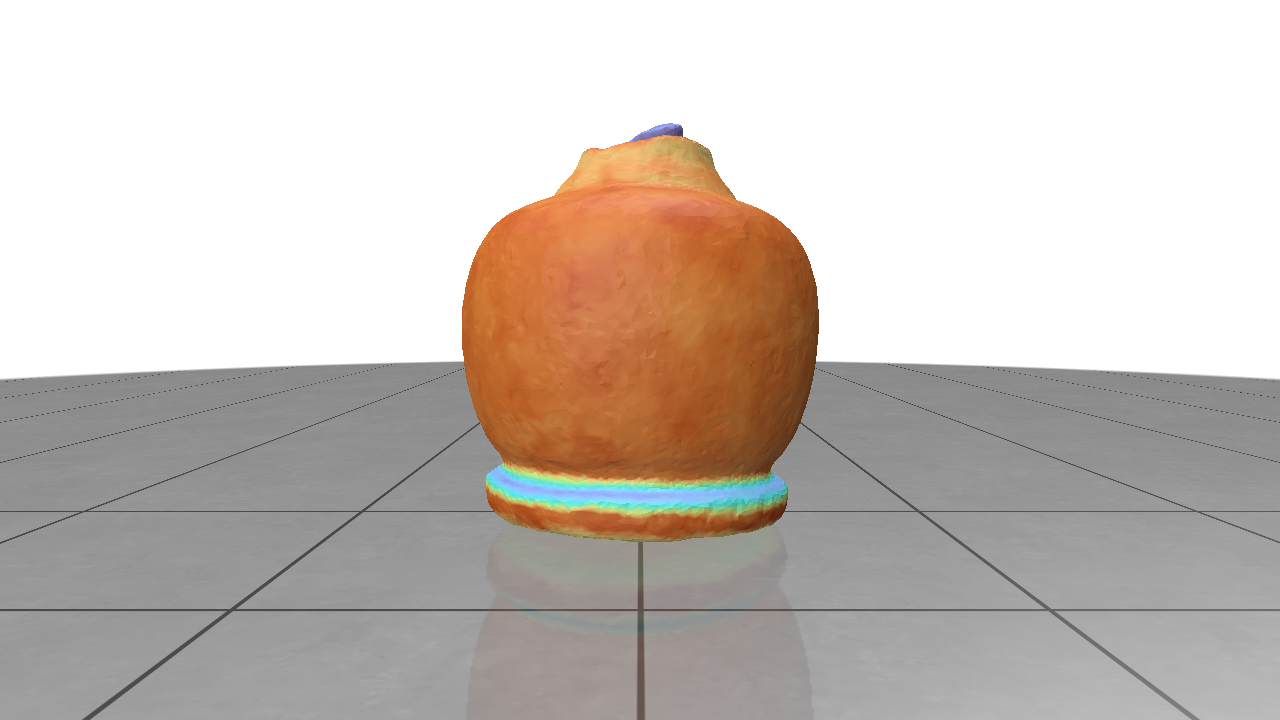
\includegraphics[width=0.65\textwidth]{../image/368_pymeshlab.png} \\
\cellcolor{blue!15}\textbf{Difference} \\
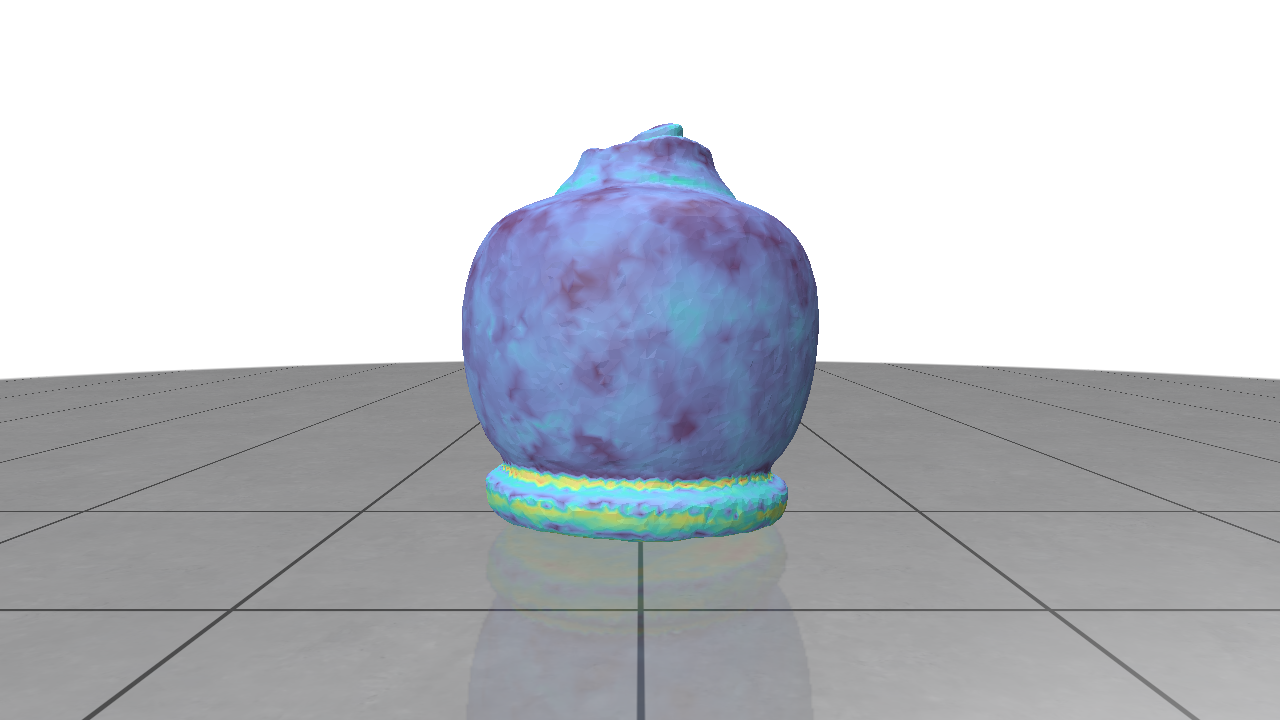
\includegraphics[width=0.65\textwidth]{../image/368_diff.png} \\
\end{tabular}
\caption{SDF quality comparison for model 368.obj (11,202 vertices)}
\label{fig:quality_368}
\end{figure}

Model 368 is a high-complexity model with 11,202 vertices. The OptiX pipeline produces a clean heat map where thick and thin regions are clearly distinguished. The PyMeshLab result shows slightly noisier transitions between regions of different thickness. The difference map reveals that the deviations are concentrated at boundary areas between thick and thin sections, where the bilateral smoothing filter in OptiX produces smoother gradients.

\begin{figure}[ht]
\centering
\begin{tabular}{@{}c@{}}
\cellcolor{red!15}\textbf{OptiX} \\
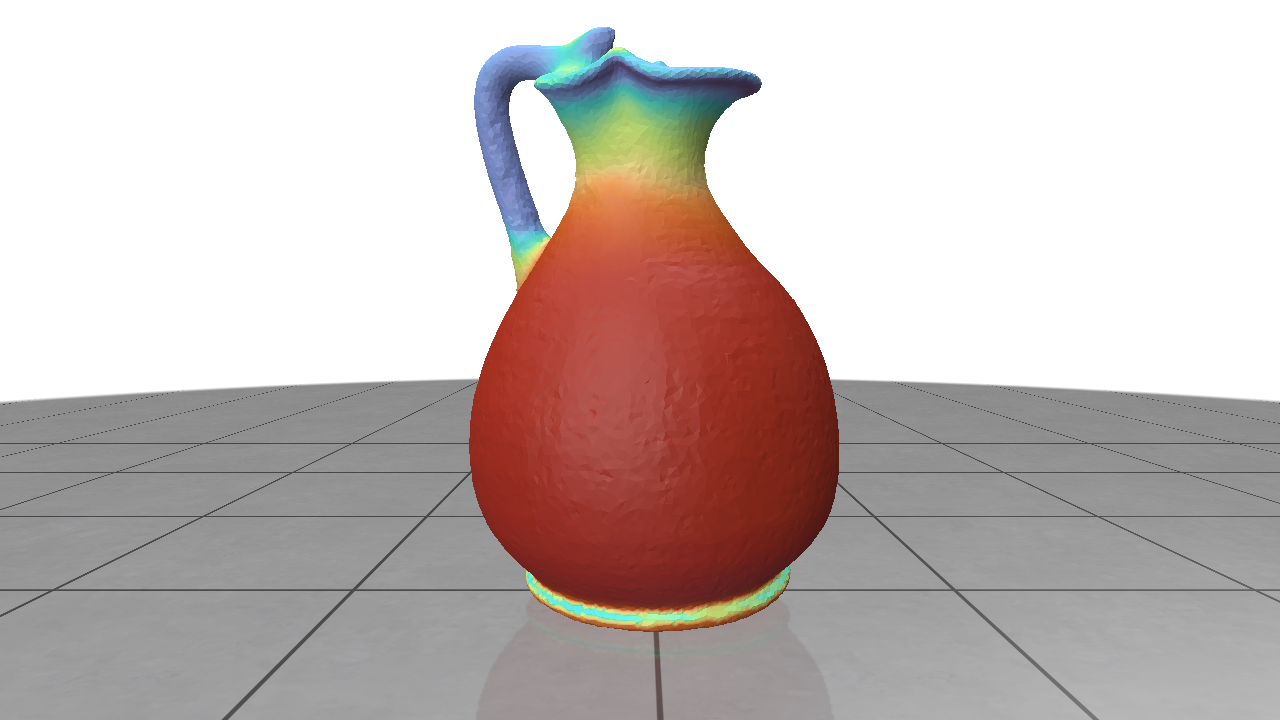
\includegraphics[width=0.65\textwidth]{../image/369_optix.png} \\
\cellcolor{green!15}\textbf{PyMeshLab} \\
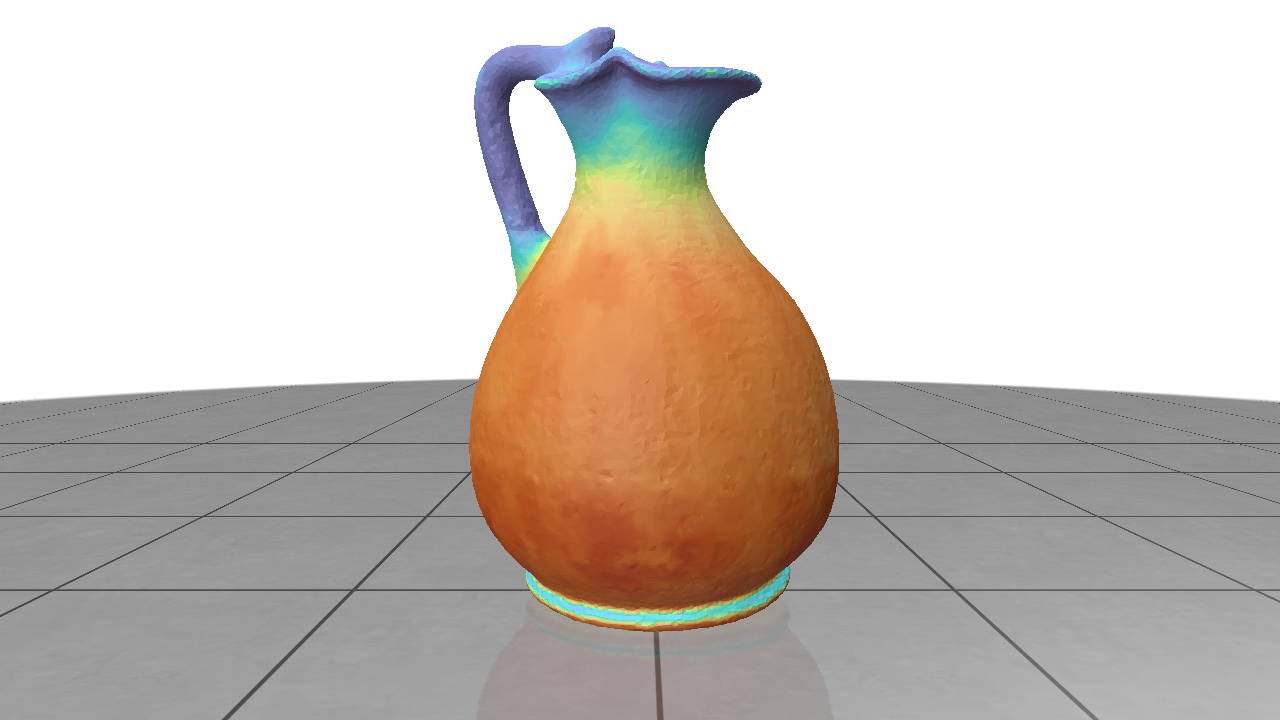
\includegraphics[width=0.65\textwidth]{../image/369_pymeshlab.png} \\
\cellcolor{blue!15}\textbf{Difference} \\
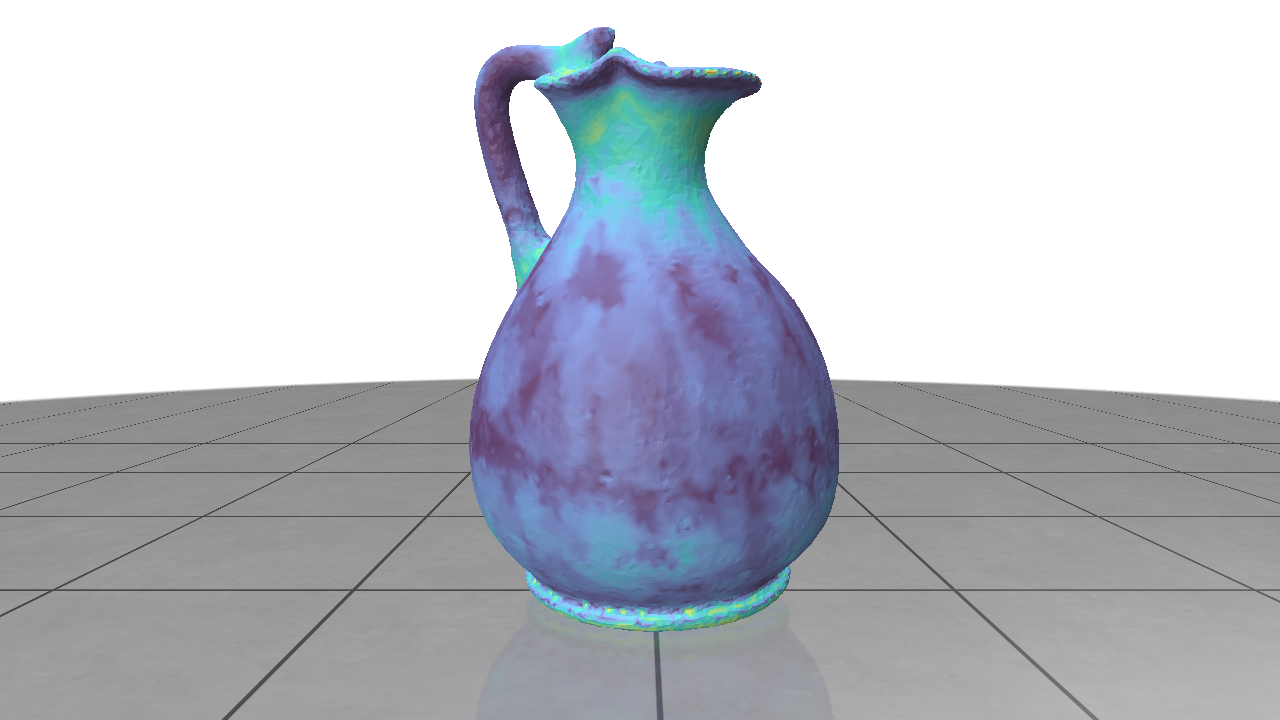
\includegraphics[width=0.65\textwidth]{../image/369_diff.png} \\
\end{tabular}
\caption{SDF quality comparison for model 369.obj (13,606 vertices)}
\label{fig:quality_369}
\end{figure}

Model 369 is comparable in size to model 112 with 13,606 vertices. The OptiX result shows well-preserved thickness features with smooth interpolation across flat surfaces. The PyMeshLab output captures the same overall structure but with more high-frequency noise. The difference map shows that both implementations produce consistent SDF values over large regions, with localized differences at fine geometric details.

\begin{figure}[ht]
\centering
\begin{tabular}{@{}c@{}}
\cellcolor{red!15}\textbf{OptiX} \\
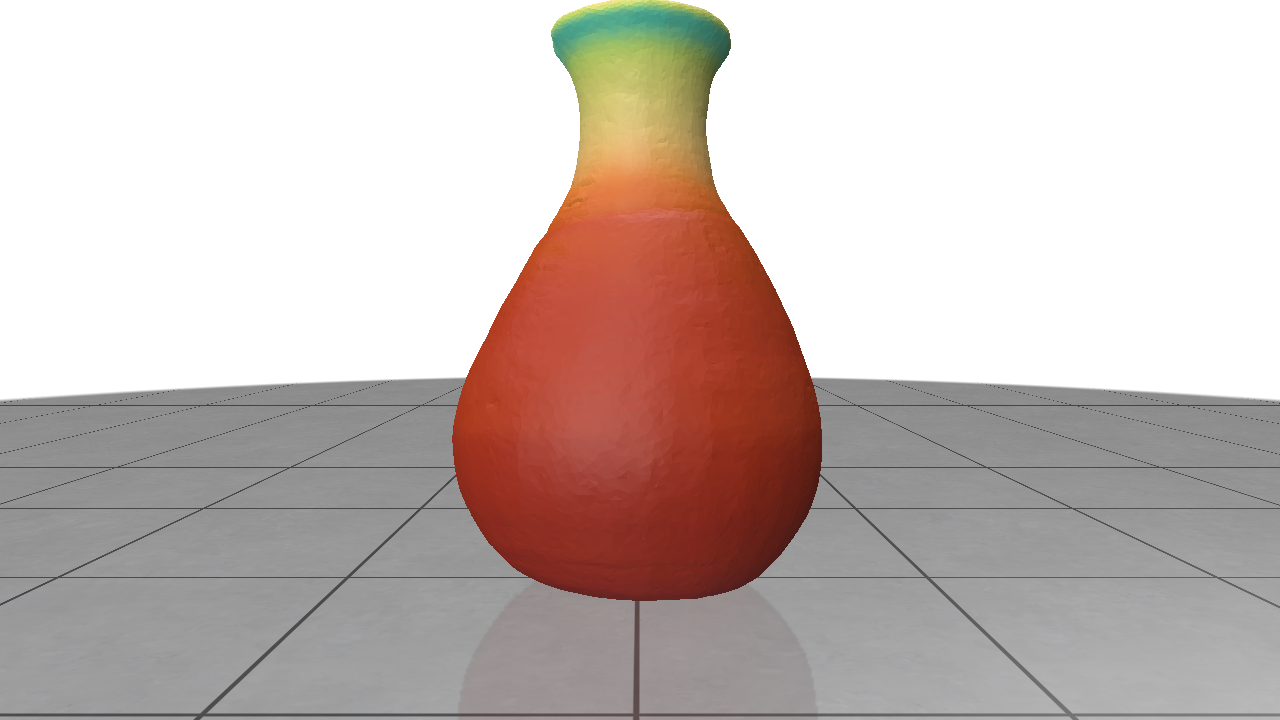
\includegraphics[width=0.65\textwidth]{../image/371_optix.png} \\
\cellcolor{green!15}\textbf{PyMeshLab} \\
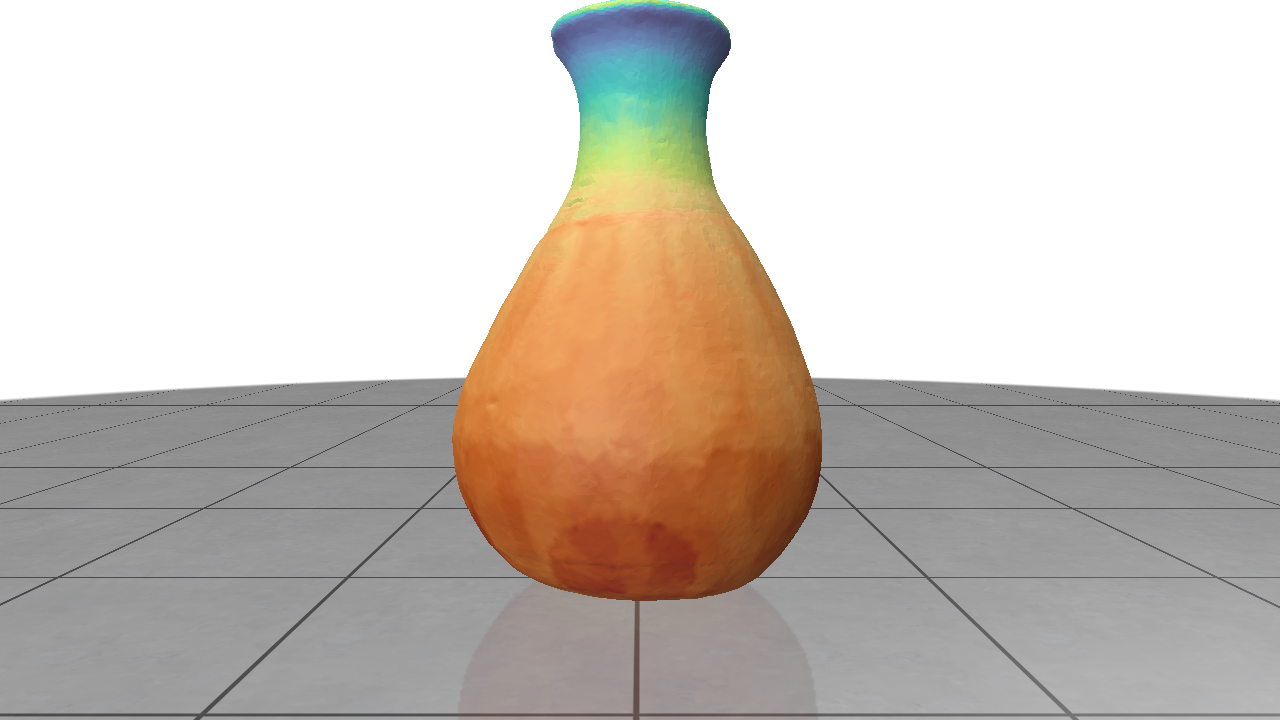
\includegraphics[width=0.65\textwidth]{../image/371_pymeshlab.png} \\
\cellcolor{blue!15}\textbf{Difference} \\
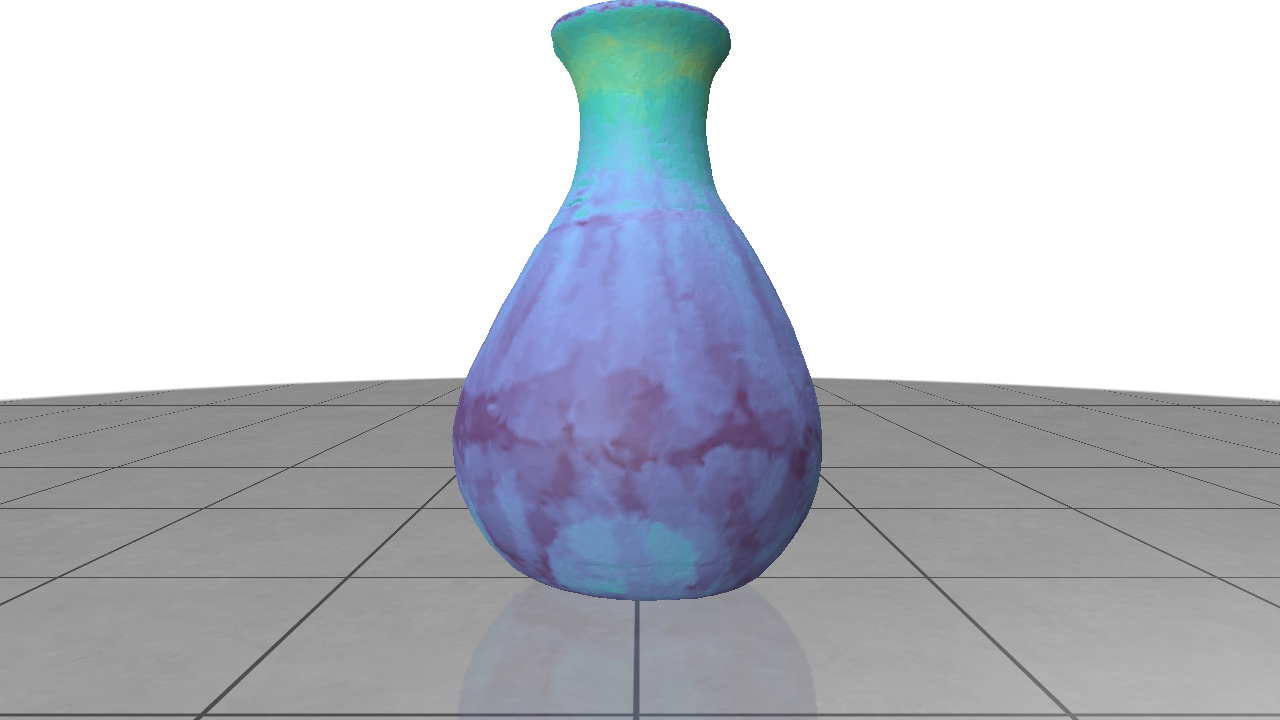
\includegraphics[width=0.65\textwidth]{../image/371_diff.png} \\
\end{tabular}
\caption{SDF quality comparison for model 371.obj (14,599 vertices)}
\label{fig:quality_371}
\end{figure}

Model 371 has the second-highest vertex count at 14,599. The OptiX heat map displays smooth, artifact-free thickness values across the entire surface. The PyMeshLab result is visually similar but exhibits minor noise in regions of uniform thickness. The difference map confirms that the two implementations produce closely matching results, with the bilateral smoothing in OptiX contributing to a cleaner output.

\begin{figure}[ht]
\centering
\begin{tabular}{@{}c@{}}
\cellcolor{red!15}\textbf{OptiX} \\
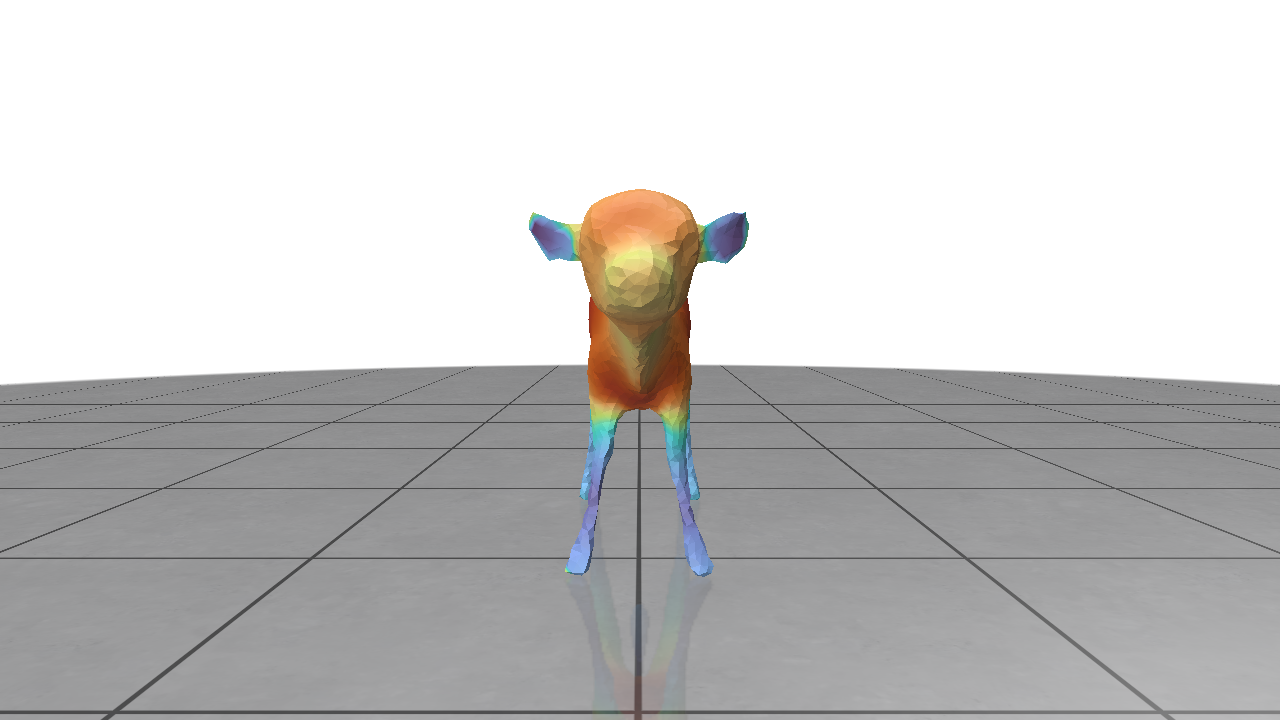
\includegraphics[width=0.65\textwidth]{../image/400_optix.png} \\
\cellcolor{green!15}\textbf{PyMeshLab} \\
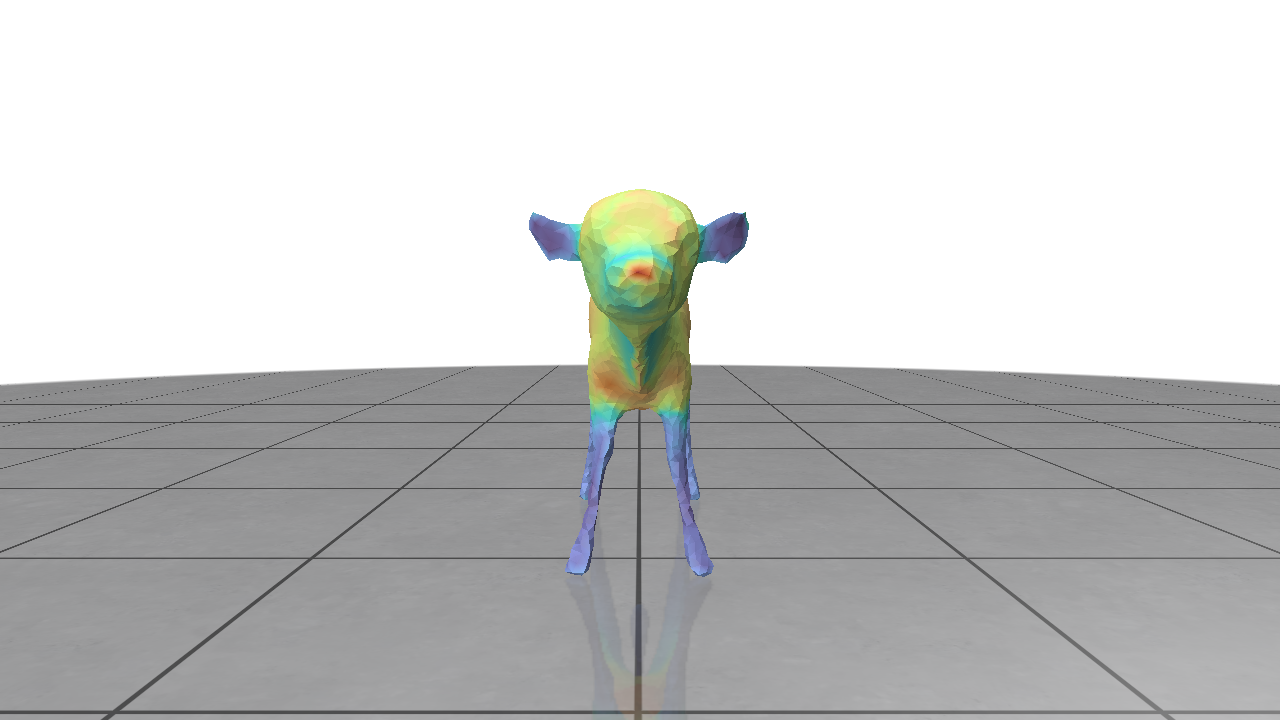
\includegraphics[width=0.65\textwidth]{../image/400_pymeshlab.png} \\
\cellcolor{blue!15}\textbf{Difference} \\
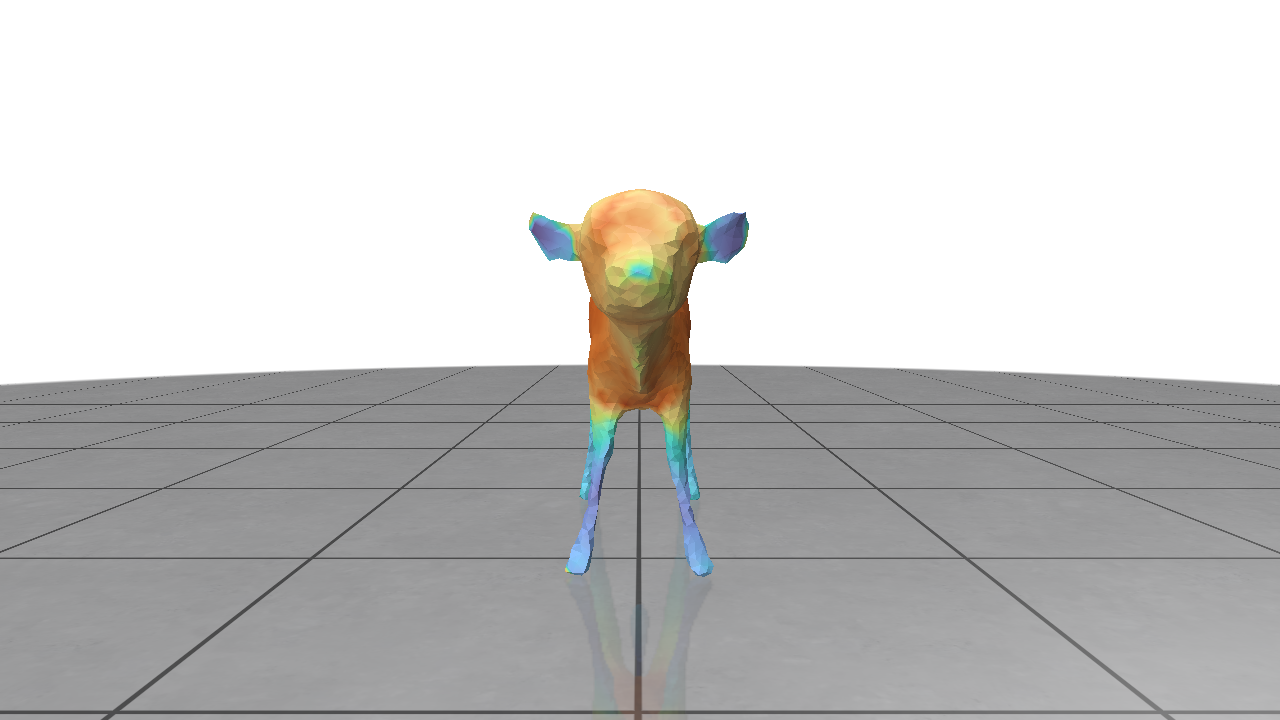
\includegraphics[width=0.65\textwidth]{../image/400_diff.png} \\
\end{tabular}
\caption{SDF quality comparison for model 400.obj (3,703 vertices)}
\label{fig:quality_400}
\end{figure}

Model 400 is a smaller model with 3,703 vertices. The OptiX heat map shows a clean, well-defined thickness distribution. The PyMeshLab result is nearly identical, with only subtle differences visible in the difference map. For small models, both implementations produce highly consistent SDF values, and the performance advantage of OptiX (33.2x speedup) does not come at the cost of quality.

\begin{figure}[ht]
\centering
\begin{tabular}{@{}c@{}}
\cellcolor{red!15}\textbf{OptiX} \\
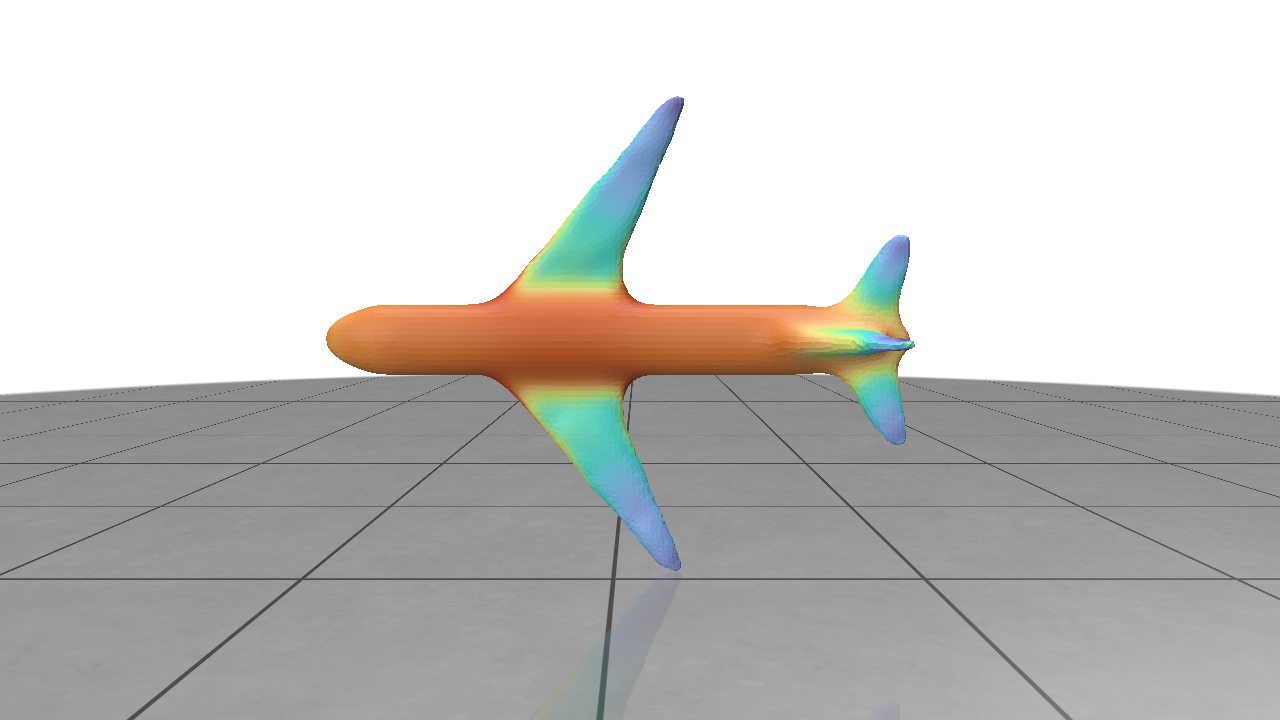
\includegraphics[width=0.65\textwidth]{../image/76_optix.png} \\
\cellcolor{green!15}\textbf{PyMeshLab} \\
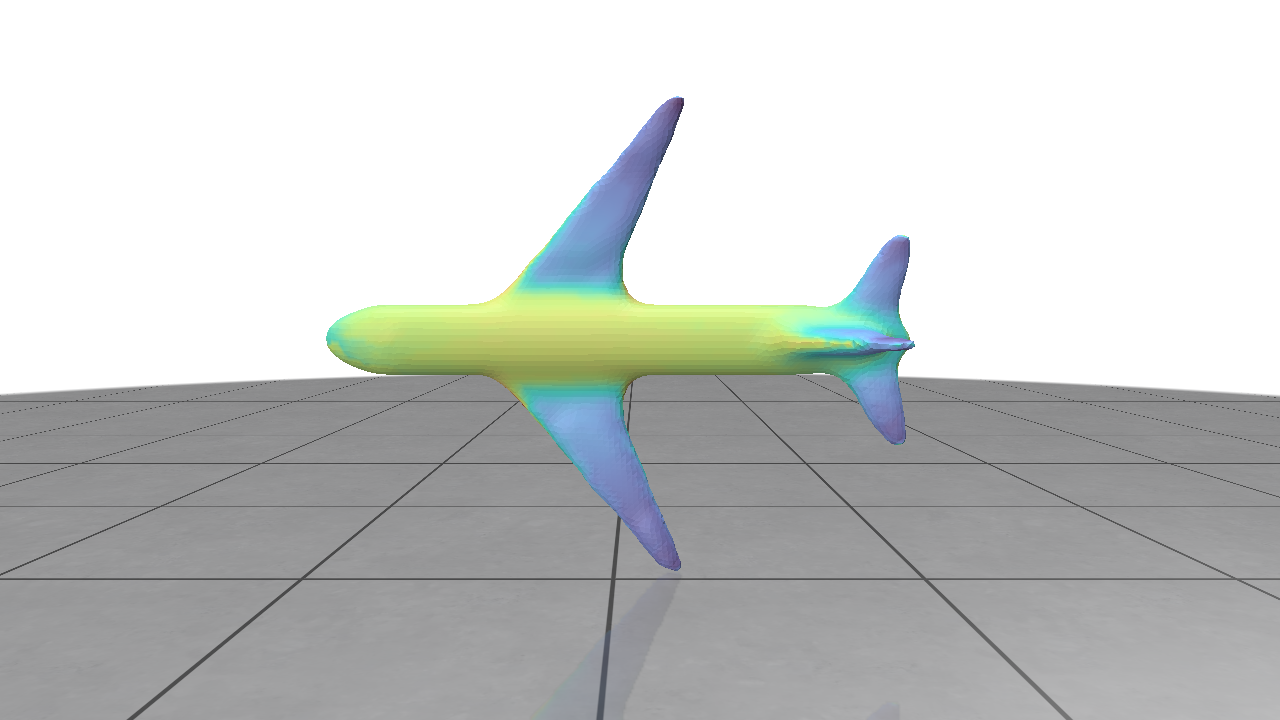
\includegraphics[width=0.65\textwidth]{../image/76_pymeshlab.png} \\
\cellcolor{blue!15}\textbf{Difference} \\
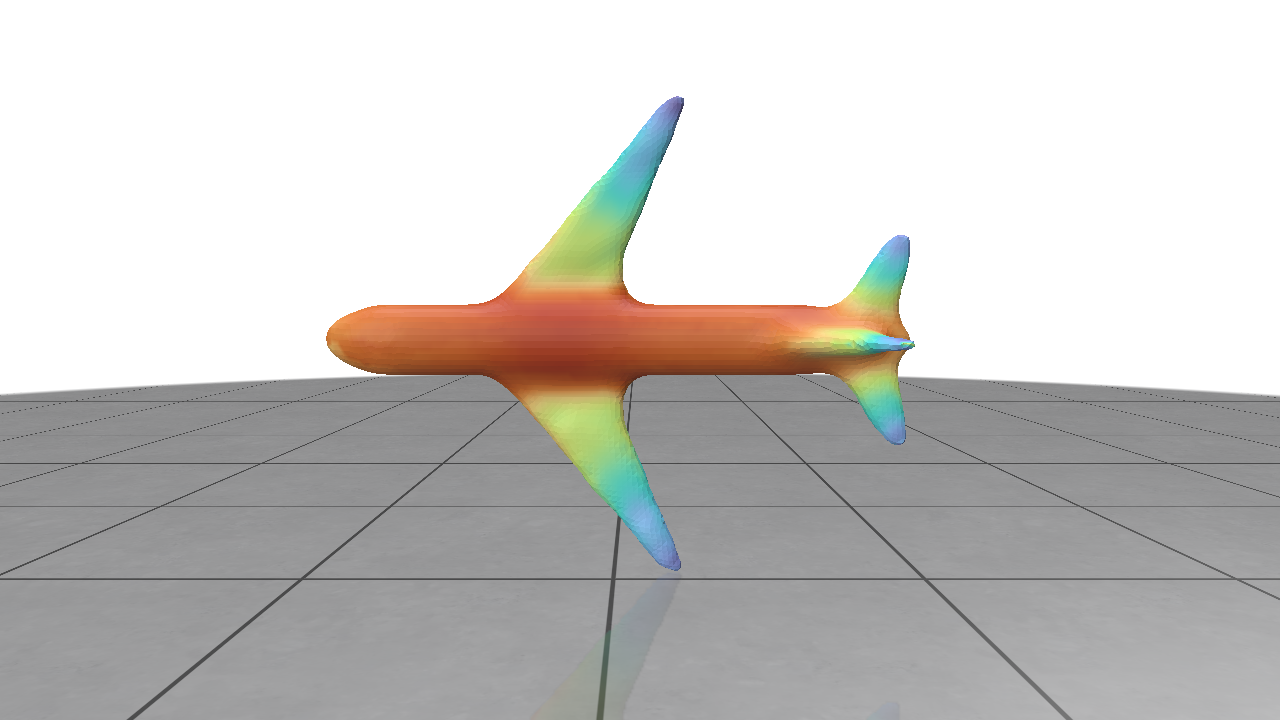
\includegraphics[width=0.65\textwidth]{../image/76_diff.png} \\
\end{tabular}
\caption{SDF quality comparison for model 76.obj (5,923 vertices)}
\label{fig:quality_76}
\end{figure}

Model 76 is a medium-complexity model with 5,923 vertices. The OptiX result shows smooth thickness transitions across the surface, while the PyMeshLab result exhibits minor noise in regions of gradual thickness change. The difference map shows that the largest deviations occur at edges and thin features, where the bilateral smoothing filter in OptiX better preserves sharp boundaries.

\begin{figure}[ht]
\centering
\begin{tabular}{@{}c@{}}
\cellcolor{red!15}\textbf{OptiX} \\
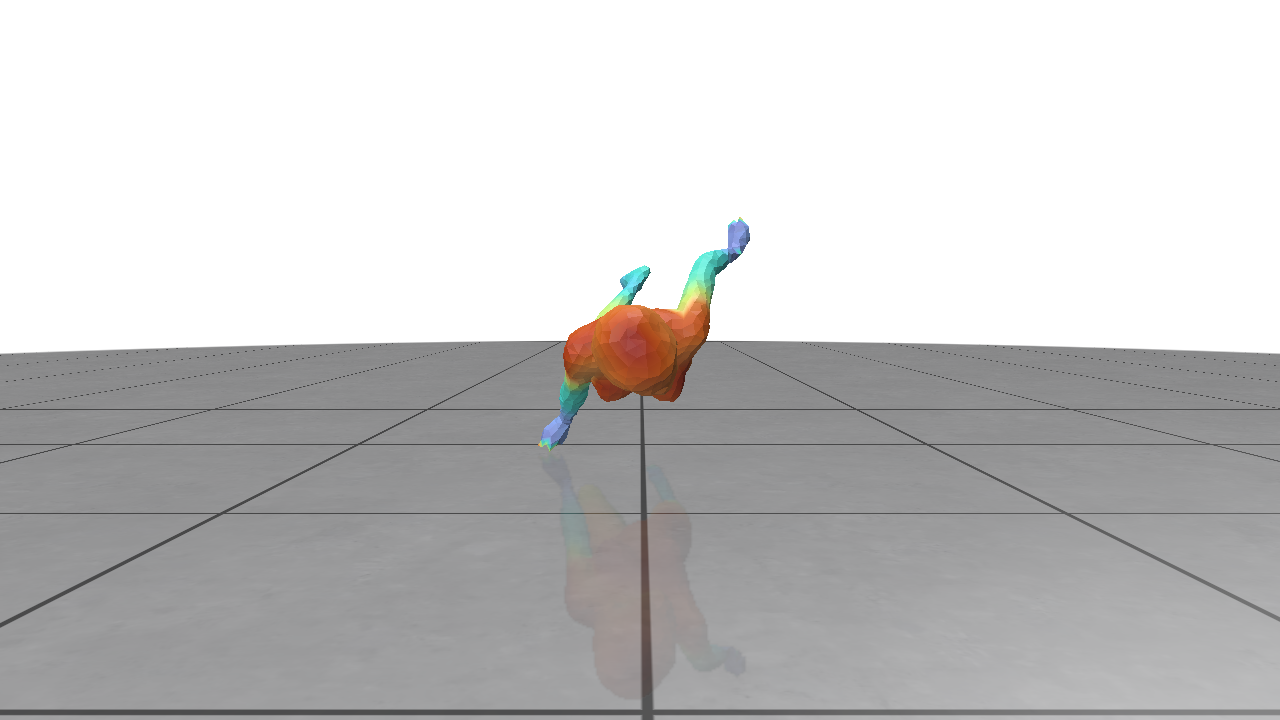
\includegraphics[width=0.65\textwidth]{../image/9_optix.png} \\
\cellcolor{green!15}\textbf{PyMeshLab} \\
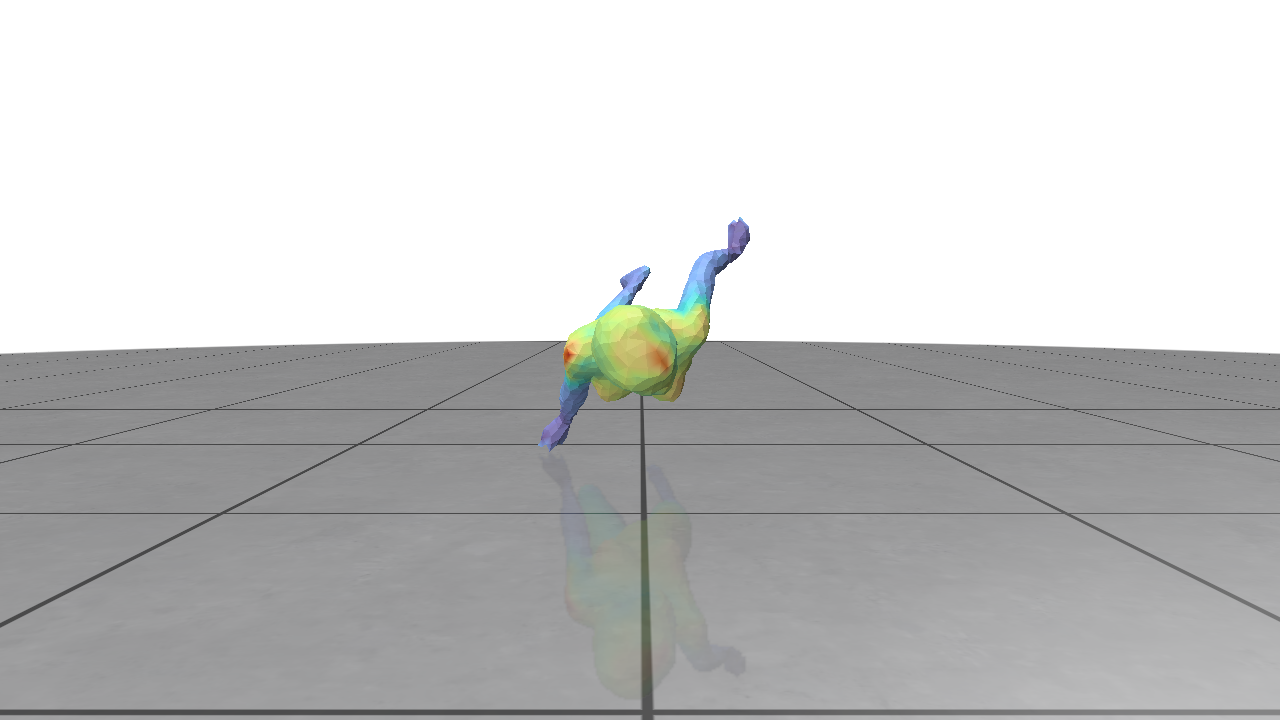
\includegraphics[width=0.65\textwidth]{../image/9_pymeshlab.png} \\
\cellcolor{blue!15}\textbf{Difference} \\
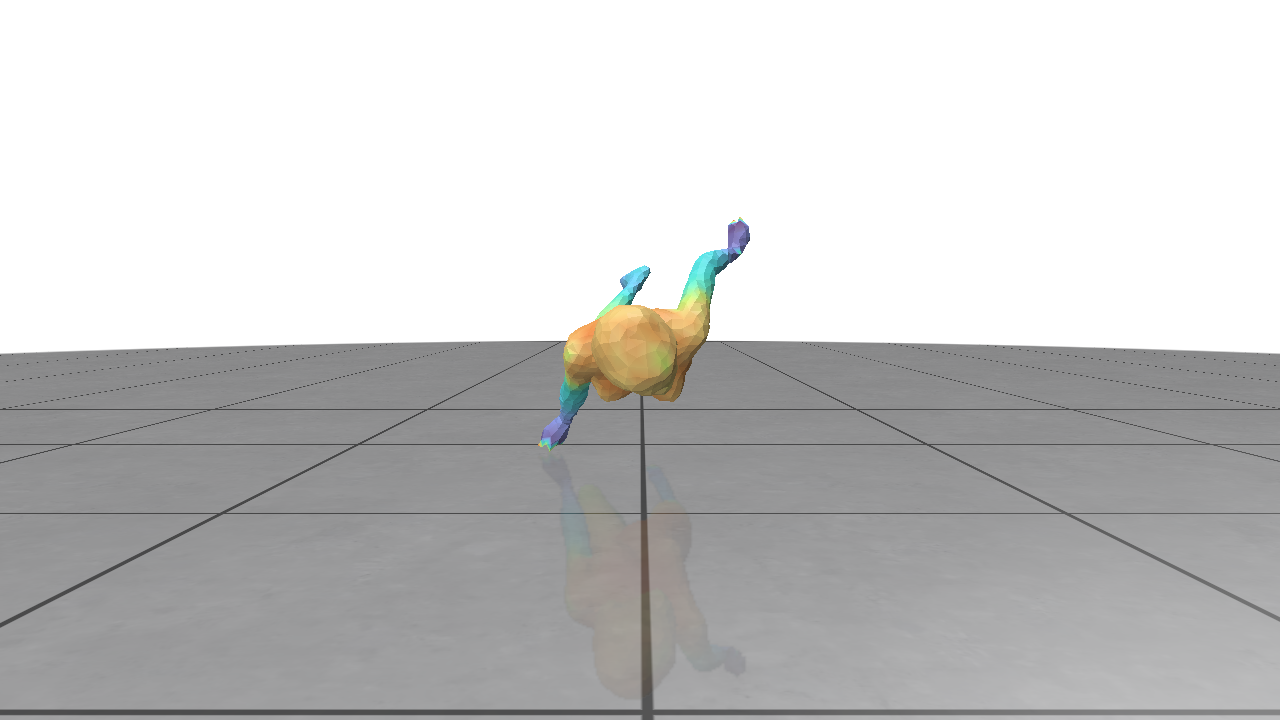
\includegraphics[width=0.65\textwidth]{../image/9_diff.png} \\
\end{tabular}
\caption{SDF quality comparison for model 9.obj (2,639 vertices)}
\label{fig:quality_9}
\end{figure}

Model 9 is the second-smallest model with only 2,639 vertices. Both implementations produce visually similar heat maps with consistent thickness values. The difference map shows minimal discrepancy, confirming that the OptiX pipeline maintains quality even for small, simple meshes. The 51.6x speedup demonstrates that OptiX provides significant performance gains across all model scales.

\clearpage

\section{Overall Conclusion}

Despite the huge difference in computation time (3.1x to 171x speedup), the OptiX SDF is still smoother than the PyMeshLab result. This is because the OptiX pipeline includes anisotropic bilateral smoothing as a post-processing step, which reduces noise while preserving sharp features. The PyMeshLab implementation produces raw SDF values without any smoothing, resulting in noisier outputs. The OptiX approach demonstrates that hardware ray tracing can simultaneously improve both performance and quality for geometric analysis tasks.
